\chapter{Implementação}

Este capítulo descreve a implementação da plataforma didática, detalhando os componentes físicos, a organização dos programas, os formatos de dados e os mecanismos empregados na reprodução, aquisição e análise dos sinais. Enquanto o capítulo anterior apresentou o procedimento metodológico, aqui são discutidas as decisões que materializam esse procedimento no computador, na ESP32 geradora e na ESP32 receptora. Para manter o texto principal concentrado nas decisões de projeto, trechos representativos de código e comandos de execução foram reunidos no Apêndice \ref{ap:comandos-execucao}.

A implementação integra três \textit{scripts} e dois \textit{firmwares} principais, identificados na Seção \ref{sec:organizacao-software}. O processamento crítico foi distribuído entre as duas ESP32: a geradora interpreta o COMTRADE e controla o DAC, enquanto a receptora adquire os sinais, estima os fasores e executa as funções de proteção. O computador permanece responsável pela preparação dos arquivos, pela configuração dos ensaios e pela supervisão da comunicação serial.

\section{Visão geral da implementação}

O encadeamento implementado pode ser dividido em três domínios. No domínio computacional, o MATLAB/Simulink gera as grandezas elétricas e o computador transfere os arquivos e os ajustes. No domínio embarcado de geração, a oscilografia é convertida em códigos temporizados para o DAC. No domínio embarcado de proteção, os sinais analógicos de tensão e corrente são novamente digitalizados e convertidos em grandezas de engenharia antes da aplicação dos algoritmos de proteção. Na Figura \ref{fig:implementacao-blocos}, a expressão ``envio das amostras'' sintetiza a transferência do registro COMTRADE completo; a cadência de reprodução não é produzida pelo Python, mas pelo \textit{firmware} gerador.

Essa separação evita que o computador participe do caminho de tempo crítico durante a reprodução ou a decisão de proteção. Depois de configuradas, as duas ESP32 executam localmente suas tarefas principais, reduzindo a dependência do escalonamento do sistema operacional e da latência da comunicação USB.

\begin{figure}[H]
  \centering
  \caption{Diagrama simplificado da implementação, destacando os principais blocos funcionais.}
  \label{fig:implementacao-blocos}
  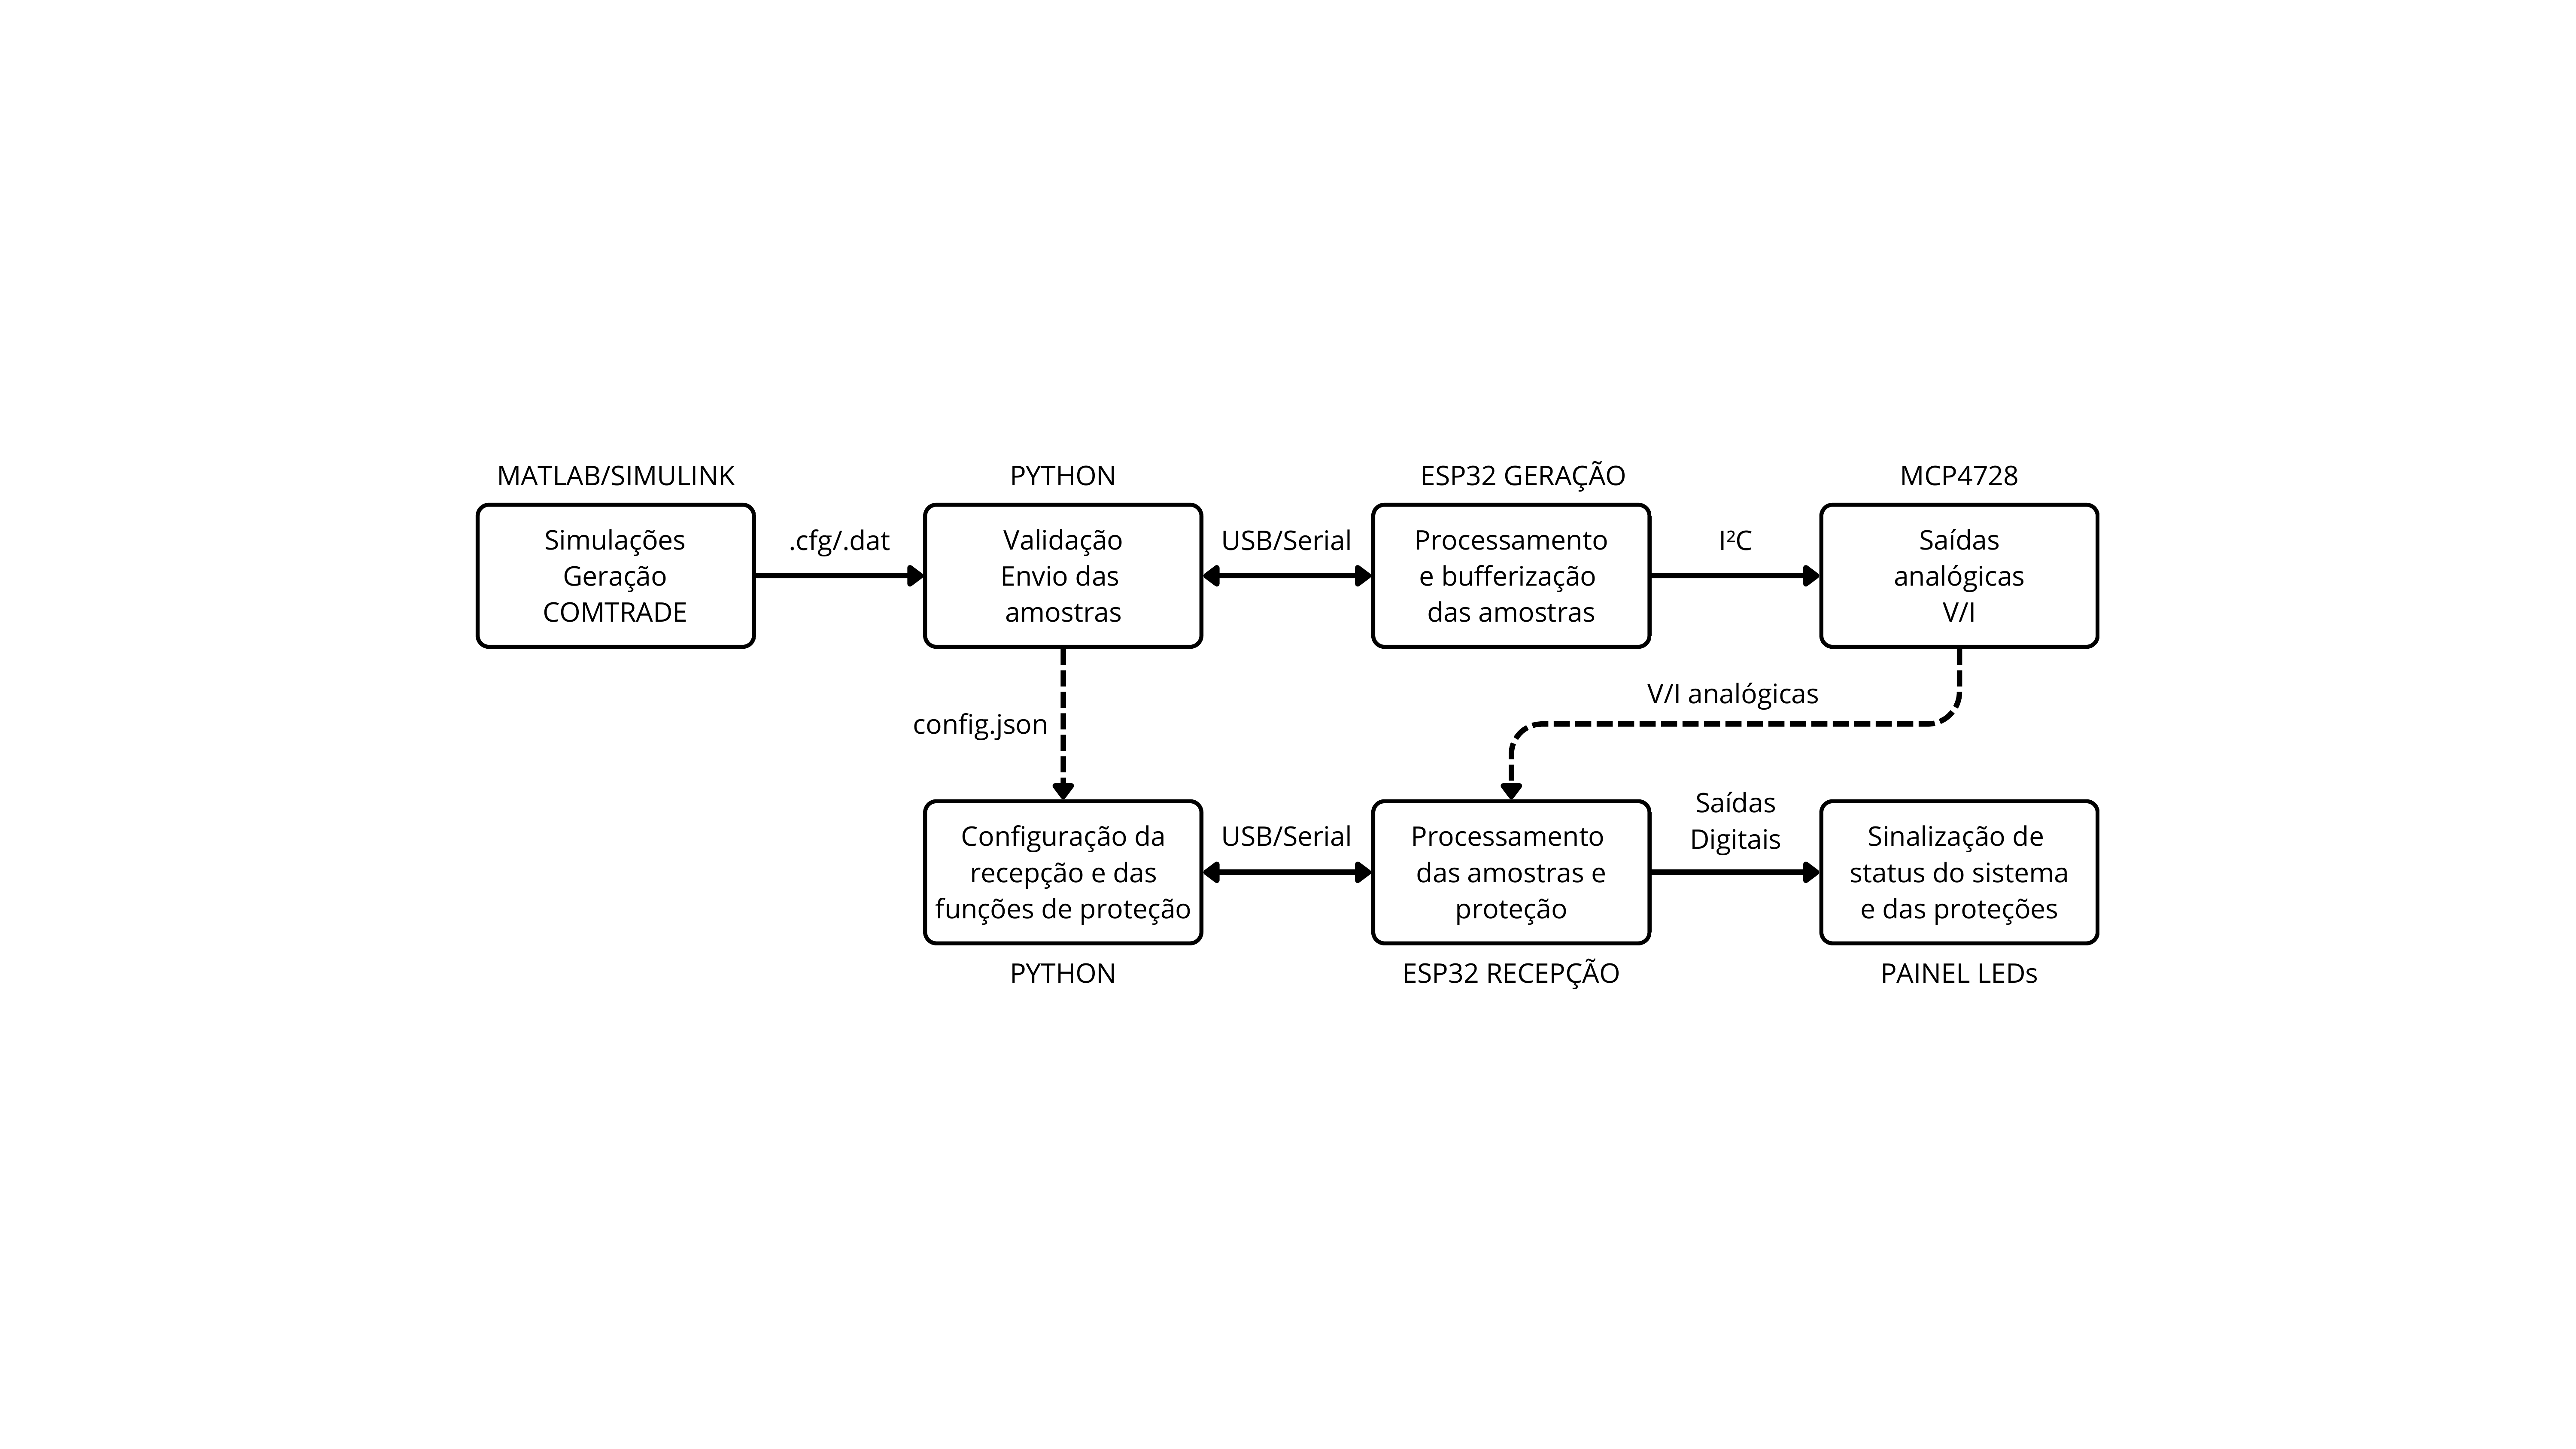
\includegraphics[
    width=\textwidth,
    trim=265pt 250pt 265pt 250pt,
    clip
  ]{figuras/diagrama_simplificado_limpo.png}
  \legend{Fonte: Autoria própria.}
\end{figure}

\section{Implementação do \textit{hardware}}

\subsection{Componentes da plataforma}

Os principais componentes são apresentados na Tabela \ref{tab:componentes-implementacao}. Foram utilizadas duas placas ESP32 independentes para que a geração e a proteção pudessem operar de forma concorrente, com recursos de processamento, memória e comunicação dedicados.

\begin{table}[H]
  \centering
  \small
  \caption{Principais componentes da plataforma.}
  \label{tab:componentes-implementacao}
  \begin{tabular}{p{3.4cm}p{9.4cm}}
    \toprule
    Componente & Função na implementação \\
    \midrule
    Computador & Executar MATLAB/Simulink e \textit{scripts} Python, armazenar os registros, transferir arquivos, enviar ajustes e exibir eventos. \\
    ESP32 geradora & Armazenar e interpretar o COMTRADE, formar os quadros temporizados e comandar o DAC. \\
    MCP4728 & Converter os códigos de 12 bits em dois sinais analógicos, um de tensão e outro de corrente. \\
    ESP32 receptora & Digitalizar os sinais, estimar a componente fundamental e executar as funções ANSI 27, 59, 50, 51, 21 e 67. \\
    LEDs/saídas digitais & Indicar estado do sistema, \textit{trip}, bloqueio, permissão e estados das zonas de distância. \\
    Protoboard e conexões & Interligar alimentação, terra comum, barramento I\textsuperscript{2}C, canais analógicos e indicadores. \\
    \bottomrule
  \end{tabular}
  \legend{Fonte: Autoria própria.}
\end{table}

\subsection{Ambiente computacional e placas utilizadas}

Os ensaios e o desenvolvimento foram realizados em um \textit{notebook} Avell A70 HYB com arquitetura x86--64, processador Intel Core i7-12700H --- 14 núcleos, 20 \textit{threads} e frequência máxima de \SI{4,7}{\giga\hertz} \cite{intel_i7_12700h} --- e \SI{16}{\gibi\byte} de memória RAM. O sistema operacional utilizado foi o Ubuntu 24.04.4 LTS (Noble Numbat), pertencente à série Ubuntu 24.04 LTS. Essa configuração corresponde especificamente ao equipamento empregado no trabalho, uma vez que o modelo A70 HYB pode ser comercializado com diferentes combinações de memória e armazenamento.

O computador executa o MATLAB/Simulink R2025b, versão utilizada na modelagem do sistema elétrico e na geração dos vetores de tempo, tensão e corrente, além dos \textit{scripts} Python, da configuração serial e do registro das mensagens. Entretanto, a reprodução temporizada e a decisão das proteções permanecem nas unidades embarcadas. Assim, a capacidade computacional do \textit{notebook} contribui para a preparação e a supervisão dos ensaios, mas não integra diretamente o caminho de tempo crítico.

Na unidade geradora foi utilizada uma placa de desenvolvimento de 38 pinos baseada no módulo ESP32-WROOM-32D, variante N4, com \SI{4}{\mebi\byte} de memória \textit{flash}. Na unidade receptora empregou-se uma placa de desenvolvimento de 30 pinos baseada no módulo ESP-WROOM-32, também com \SI{4}{\mebi\byte} de \textit{flash}. A quantidade de pinos mencionada descreve os conectores disponíveis em cada placa de desenvolvimento e não deve ser confundida com a quantidade total de GPIOs do circuito integrado.

Os dois módulos pertencem à família ESP32 e utilizam processador Xtensa LX6 de 32 bits com dois núcleos e frequência de até \SI{240}{\mega\hertz}, além de \SI{520}{\kibi\byte} de SRAM e interfaces UART, SPI e I\textsuperscript{2}C. O circuito integrado possui dois conversores SAR: o ADC1 dispõe de oito canais e o ADC2 de dez, totalizando até 18 entradas analógicas multiplexadas, com resolução configurável e valor nominal de 12 bits, correspondente a 4096 códigos. A quantidade efetivamente acessível depende dos GPIOs expostos pela placa de desenvolvimento. Neste projeto, a receptora emprega somente duas entradas do ADC1, GPIO35 para tensão e GPIO34 para corrente, ambas configuradas por \texttt{analogReadResolution(12)} e com atenuação \texttt{ADC\_11db}. O uso do ADC1 também mantém a aquisição independente dos canais do ADC2, compartilhados com o subsistema Wi-Fi do ESP32. O ESP32-WROOM-32D opera com alimentação do módulo entre \SIrange{3,0}{3,6}{\volt} e possui antena de placa integrada \cite{espressif_wroom32d,espressif_wroom32}.

O ESP32 dispõe nativamente de somente duas saídas DAC, associadas aos GPIO25 e GPIO26, com resolução de 8 bits, isto é, 256 códigos. Para a geração foi adotado o MCP4728, conversor digital-analógico externo de quatro canais e 12 bits, controlado por I\textsuperscript{2}C e dotado de memória não volátil. A escolha eleva a discretização para 4096 códigos --- 16 vezes mais níveis que o DAC interno --- e permite controlar quatro saídas por uma única interface digital, preservando dois canais para tensão e corrente e dois canais para expansão. Considerando a referência de \SI{3,3}{\volt}, o incremento ideal passa de aproximadamente \SI{12,9}{\milli\volt}, no DAC interno de 8 bits, para cerca de \SI{0,81}{\milli\volt} no MCP4728. Essa resolução mais fina reduz os degraus de quantização na reconstrução das oscilografias e justifica o conversor externo mesmo quando apenas dois canais são reproduzidos. Nesta plataforma, os canais A e B reproduzem, respectivamente, tensão e corrente, enquanto C e D permanecem no nível de repouso \cite{microchip_mcp4728}.

\begin{table}[H]
  \centering
  \small
  \caption{Configuração computacional e placas empregadas na plataforma.}
  \label{tab:ambiente-computacional}
  \begin{tabular}{p{3.6cm}p{9.2cm}}
    \toprule
    Elemento & Configuração utilizada \\
    \midrule
    Computador & Avell A70 HYB; Intel Core i7-12700H; 14 núcleos e 20 \textit{threads}; \SI{16}{\gibi\byte} de RAM; arquitetura x86--64. \\
    Sistema operacional & Ubuntu 24.04.4 LTS, codinome Noble Numbat \cite{ubuntu_2404}. \\
    Simulação & MATLAB/Simulink R2025b, utilizado na modelagem e na geração das amostras. \\
    Unidade geradora & Placa de desenvolvimento de 38 pinos; ESP32-WROOM-32D N4; dois núcleos LX6 de até \SI{240}{\mega\hertz}; \SI{4}{\mebi\byte} de \textit{flash}. \\
    Conversor D/A & MCP4728; quatro canais; 12 bits; interface I\textsuperscript{2}C; alimentação de \SI{3,3}{\volt}. \\
    Unidade receptora & Placa de desenvolvimento de 30 pinos; ESP-WROOM-32; dois núcleos LX6 de até \SI{240}{\mega\hertz}; \SI{4}{\mebi\byte} de \textit{flash}; até 18 canais ADC SAR de 12 bits no circuito integrado; GPIO34 e GPIO35 utilizados. \\
    \bottomrule
  \end{tabular}
  \legend{Fonte: Autoria própria, com dados técnicos dos fabricantes.}
\end{table}

\subsection{Unidade geradora e DAC}

Na unidade geradora, o MCP4728 é controlado por I\textsuperscript{2}C no endereço \texttt{0x60}. O GPIO21 da ESP32 é utilizado como SDA e o GPIO22 como SCL. O barramento foi configurado em \SI{1}{\mega\hertz}, valor adotado para reduzir o tempo de atualização do conversor durante a reprodução. O canal A do MCP4728 recebe os códigos de tensão, o canal B os códigos de corrente, e os canais C e D permanecem no código central de repouso.

O DAC possui resolução de 12 bits, de modo que sua faixa digital contém 4096 códigos. A referência usada no \textit{firmware} é \SI{3,3}{\volt}; assim, o código central 2048 produz aproximadamente \SI{1,65}{\volt}. Esse nível é utilizado tanto como ponto de repouso quanto como deslocamento de nível das formas de onda alternadas.

\begin{table}[H]
  \centering
  \small
  \caption{Conexões da unidade geradora.}
  \label{tab:pinagem-geradora}
  \begin{tabular}{lll}
    \toprule
    Elemento & Conexão & Finalidade \\
    \midrule
    ESP32 GPIO21 & MCP4728 SDA & Dados do barramento I\textsuperscript{2}C \\
    ESP32 GPIO22 & MCP4728 SCL & Relógio do barramento I\textsuperscript{2}C \\
    MCP4728 canal A & Entrada de tensão da receptora & Reprodução de $V$ \\
    MCP4728 canal B & Entrada de corrente da receptora & Reprodução de $I$ \\
    MCP4728 canais C/D & Código 2048 & Canais não utilizados \\
    GND da geradora & GND da receptora & Referência comum dos sinais \\
    \bottomrule
  \end{tabular}
  \legend{Fonte: Autoria própria.}
\end{table}

O aspecto físico dessa unidade foi apresentado anteriormente na Figura \ref{fig:unidade-geradora}, no capítulo de Metodologia. Nesta seção, a ênfase recai sobre suas conexões e decisões de implementação, evitando a repetição da mesma fotografia.

\subsection{Unidade receptora e sinalização}

O \textit{firmware} receptor configura os GPIOs 35 e 34 como entradas analógicas de tensão e corrente, respectivamente. A resolução do ADC é de 12 bits e a atenuação de \SI{11}{\decibel} é habilitada para compatibilizar a faixa de entrada com a saída do DAC. A correspondência de canais adotada no \textit{firmware} é, portanto, GPIO35 para tensão e GPIO34 para corrente.

A ESP32 receptora executa todas as funções de proteção implementadas na plataforma: sobrecorrente instantânea (ANSI 50), sobrecorrente temporizada (ANSI 51), subtensão (ANSI 27), sobretensão (ANSI 59), distância (ANSI 21) e supervisão direcional (ANSI 67). Essas funções podem ser habilitadas ou desabilitadas individualmente pelo \textit{script} de configuração e são avaliadas a partir dos mesmos fasores fundamentais de tensão e corrente.

As quatro saídas digitais GPIO14, GPIO27, GPIO26 e GPIO25 representam estados agregados da hierarquia de proteção. As duas primeiras indicam bloqueio e permissão da supervisão 67. O GPIO26 reúne os trips instantâneos produzidos pela zona 1 da função 21, pelo estágio instantâneo das funções 27 e 59 e pela função 50. O GPIO25 reúne os trips temporizados da zona 2 da função 21, dos estágios temporizados das funções 27 e 59 e da função 51. Assim, o significado das duas últimas indicações depende das proteções habilitadas no ensaio; a origem específica permanece discriminada pelas mensagens seriais. Quando a função 67 está habilitada, sua condição direcional autoriza ou bloqueia esses trips conforme a hierarquia apresentada na Seção \ref{sec:hierarquia-protecoes}.

As funções 27, 59, 50 e 51 são identificadas nominalmente pelas mensagens de eventos na interface serial e também contribuem para o sinal geral de \textit{trip} indicado pelo GPIO12. Dessa forma, a indicação geral do painel é complementada pelo detalhamento fornecido no terminal.

O GPIO13 indica que o sistema está pronto, enquanto o GPIO12 pisca quando existe qualquer \textit{trip} retido, independentemente de sua origem. As saídas foram implementadas como ativas em nível alto; essa escolha deve ser revista caso seja empregado um módulo de relés com entradas ativas em nível baixo.

\begin{table}[H]
  \centering
  \small
  \caption{Pinagem implementada na ESP32 receptora.}
  \label{tab:pinagem-receptora}
  \begin{tabular}{cll}
    \toprule
    GPIO & Tipo & Função \\
    \midrule
    35 & Entrada ADC & Canal de tensão \\
    34 & Entrada ADC & Canal de corrente \\
    14 & Saída digital & Bloqueio imposto pela supervisão 67 \\
    27 & Saída digital & Permissão/habilitação fornecida pela supervisão 67 \\
    26 & Saída digital & Trip instantâneo: 21/Z1, 27, 50 ou 59 \\
    25 & Saída digital & Trip temporizado: 21/Z2, 27, 51 ou 59 \\
    13 & Saída digital & Estado de prontidão do sistema \\
    12 & Saída digital & Trip retido por 27, 59, 50, 51 ou 21 \\
    \bottomrule
  \end{tabular}
  \legend{Fonte: Autoria própria.}
\end{table}

A interligação física adotada segue o mapa compilado no \textit{firmware} receptor: tensão no GPIO35 e corrente no GPIO34. O JSON fornece as escalas e os valores de referência associados a esses canais, preservando a correspondência entre as grandezas reproduzidas e adquiridas. Como a reconstrução final depende do ganho efetivo do DAC, da entrada ADC e da montagem física, o \textit{script} receptor também admite fatores multiplicativos de correção de escala. Esses fatores são aplicados sobre as escalas do JSON antes do envio à ESP32 receptora e permitem ajustar a leitura de pré-falta aos valores nominais do registro.

As fotografias da unidade receptora e do painel de sinalização já foram apresentadas nas Figuras \ref{fig:unidade-receptora} e \ref{fig:indicacao-leds}, no capítulo de Metodologia. A Tabela \ref{tab:pinagem-receptora} complementa essas imagens com a associação funcional dos terminais.

\subsection{Cuidados elétricos da interligação}

Os sinais da bancada estão limitados à faixa de baixa tensão e não são conectados diretamente ao sistema de \SI{500}{\kilo\volt} modelado. As grandezas de potência existem apenas como valores de engenharia associados às formas de onda. A ligação DAC--ADC exige terra comum, verificação da polaridade, ausência de curto-circuitos e garantia de que a tensão permaneça na faixa admitida pelas entradas da ESP32.

Embora a montagem em protoboard seja adequada ao protótipo didático, uma versão consolidada deve acrescentar resistores em série, desacoplamento próximo às placas, conectores identificados e pontos de teste. Também é recomendável documentar a ligação em um diagrama elétrico com os canais A/B do DAC, GPIO35/GPIO34, alimentação e terra. Esse esquema não aparece na arquitetura funcional, mas é importante para a reprodução do experimento por terceiros.

\section{Organização do \textit{software}}
\label{sec:organizacao-software}

\begin{table}[H]
  \centering
  \small
  \caption{Arquivos principais e responsabilidades efetivamente implementadas.}
  \label{tab:arquivos-software}
  \begin{tabular}{p{4.0cm}p{8.8cm}}
    \toprule
    Arquivo & Responsabilidade \\
    \midrule
    \path{generate_comtrade.m} & Extrair os vetores do MATLAB, gerar gráficos e produzir um COMTRADE ASCII trifásico inicial. \\
    \path{run_embedded_generator.py} & Transferir o \texttt{.cfg} e o \texttt{.bdat}, solicitar o processamento, gerar o JSON e oferecer o terminal de reprodução. \\
    \path{embedded_generator.ino} & Armazenar os arquivos, interpretar o COMTRADE binário, calcular escalas, criar quadros e atualizar o MCP4728. \\
    \path{config.json} & Vincular o registro processado às escalas, valores nominais, frequência, taxa de amostragem e recomendações da recepção. \\
    \path{run_embedded_receiver.py} & Ler o JSON, combinar seus dados com os ajustes de proteção e configurar a ESP32 receptora. \\
    \path{embedded_receiver.ino} & Adquirir os canais, remover \textit{offset}, estimar fasores, avaliar proteções e controlar as saídas. \\
    \bottomrule
  \end{tabular}
  \legend{Fonte: Autoria própria.}
\end{table}

O código-fonte completo, incluindo \textit{scripts} Python, \textit{firmwares}, arquivos de apoio e histórico de desenvolvimento, está disponível no repositório público \textit{TCC\_master}, hospedado no GitHub em \url{https://github.com/paulotaraujo/TCC_master} \cite{pereira_tcc_master_2026}. O Apêndice \ref{ap:comandos-execucao} apresenta apenas os trechos necessários para evidenciar as decisões centrais de implementação e os comandos de reprodução dos ensaios; por isso, deve ser lido como uma referência operacional resumida, e não como substituto da consulta ao repositório completo.

\subsection{Bibliotecas, dependências e ambiente de compilação}

As interfaces Python foram implementadas com o PySerial 3.5 como dependência externa para a comunicação USB/serial. Nos \textit{scripts} \path{run_embedded_generator.py} e \path{run_embedded_receiver.py}, esse pacote realiza a abertura da porta, a transmissão de comandos e dados e a recepção das respostas das placas. Sua instalação pode ser realizada com o comando \texttt{python3 -m pip install pyserial}. As demais funcionalidades utilizam módulos da biblioteca padrão do Python: \texttt{argparse} processa os argumentos da linha de comando; \texttt{json} trata o arquivo de configuração; \texttt{sys} e \texttt{time} apoiam o controle da execução; e \texttt{pathlib} e \texttt{typing} organizam os caminhos e as interfaces do código. Na geração, \texttt{math} executa os cálculos numéricos e \texttt{threading} mantém a leitura serial concorrente com o terminal interativo. Essa organização concentra as dependências externas na camada de comunicação e utiliza os recursos nativos do Python nas demais tarefas.

O ambiente de compilação dos \textit{firmwares} foi padronizado com o núcleo \texttt{esp32:esp32} 3.3.8. Esse núcleo fornece \texttt{Arduino.h} e os recursos de GPIO, ADC, temporização e comunicação serial utilizados nas duas placas. Na unidade geradora, \texttt{Wire.h} implementa o barramento I\textsuperscript{2}C; \texttt{LittleFS.h} fornece o sistema de arquivos interno usado para armazenar o \texttt{.cfg} e o \texttt{.bdat}; \texttt{esp\_heap\_caps.h} permite consultar e alocar memória com capacidades específicas; e os cabeçalhos \texttt{FreeRTOS.h}, \texttt{task.h} e \texttt{semphr.h} disponibilizam tarefas, escalonamento e sincronização. Todos esses componentes integram o núcleo Arduino-ESP32, o que mantém uma versão comum da plataforma para a geradora e a receptora.

O controle do conversor externo é realizado pela biblioteca Adafruit MCP4728 1.0.10, responsável pela inicialização e pela atualização dos quatro canais do DAC. A biblioteca utiliza a Adafruit BusIO 1.17.4 como dependência para a abstração da comunicação com o dispositivo. No \textit{firmware} receptor, \texttt{Arduino.h} fornece a infraestrutura embarcada, enquanto \texttt{math.h}, pertencente à biblioteca matemática de C/C++, disponibiliza as operações trigonométricas e algébricas empregadas na estimação fasorial e nas lógicas de proteção. A Tabela \ref{tab:bibliotecas-software} reúne as bibliotecas e versões adotadas na implementação.

\begin{table}[H]
  \centering
  \small
  \caption{Bibliotecas e dependências adotadas na implementação.}
  \label{tab:bibliotecas-software}
  \begin{tabular}{p{3.1cm}p{3.5cm}p{6.0cm}}
    \toprule
    Componente & Biblioteca ou módulo & Finalidade na plataforma \\
    \midrule
    Interfaces Python & PySerial 3.5 & Comunicação USB/serial bidirecional com as duas ESP32. \\
    Interfaces Python & Biblioteca padrão & Argumentos, JSON, arquivos, temporização, tipagem, cálculos e concorrência. \\
    Firmware gerador & Arduino-ESP32 3.3.8 & Arduino, I\textsuperscript{2}C, LittleFS, memória e FreeRTOS. \\
    Firmware gerador & Adafruit MCP4728 1.0.10 & Controle do DAC MCP4728; utiliza Adafruit BusIO 1.17.4. \\
    Firmware receptor & Arduino-ESP32 e \texttt{math.h} & ADC, GPIO, serial, temporização, cálculos fasoriais e proteções. \\
    \bottomrule
  \end{tabular}
  \legend{Fonte: Autoria própria.}
\end{table}

\section{Geração e adequação dos arquivos COMTRADE}

O \textit{script} MATLAB lê \texttt{Vin.Time}, as três colunas de \texttt{Vin.Data} e as três colunas de \texttt{Iin.Data}. A taxa de amostragem é estimada por

\begin{equation}
  f_s=\left[\frac{1}{N-1}\sum_{k=1}^{N-1}\left(t[k]-t[k-1]\right)\right]^{-1}.
\end{equation}

Além de gerar os gráficos trifásicos, o \textit{script} escreve um arquivo \texttt{.cfg} com seis canais analógicos e um arquivo \texttt{.dat} ASCII. Os coeficientes $a=1$ e $b=0$ escritos nesse arquivo indicam que os valores já se encontram em unidades de engenharia.

Entretanto, o processador COMTRADE implementado em \path{embedded_generator.ino} aceita apenas o formato \texttt{BINARY}. Os arquivos efetivamente usados nos testes são pares \texttt{export.cfg}/\texttt{export.bdat}, com dois canais analógicos ordenados como tensão e corrente. Portanto, entre a saída original do MATLAB e o \textit{upload} existe uma etapa de exportação ou conversão para binário e de seleção da fase. Essa etapa deve ser mantida documentada, pois o \textit{firmware} interpreta obrigatoriamente o primeiro canal como tensão e o segundo como corrente, independentemente dos nomes declarados no \texttt{.cfg}; exemplos de arquivos e rotinas auxiliares estão disponíveis no repositório do projeto.

O \textit{parser} embarcado lê no máximo 160 linhas do \texttt{.cfg}, extrai o número de canais, os coeficientes $a$ e $b$ dos dois primeiros canais, a frequência, a primeira taxa de amostragem, o formato e o multiplicador de tempo. O valor bruto de cada canal é convertido por

\begin{equation}
  x_{\mathrm{eng}}=a x_{\mathrm{raw}}+b.
  \label{eq:comtrade-conversao}
\end{equation}

O \textit{layout} do arquivo binário é inferido a partir do tamanho total. Para marcas de tempo de 32 bits, cada registro ocupa

\begin{equation}
  L_{32}=4+4+2N_A+2\left\lceil\frac{N_D}{16}\right\rceil \quad \text{bytes},
\end{equation}

em que $N_A$ e $N_D$ são as quantidades de canais analógicos e digitais. Para marcas de tempo de 64 bits, o segundo termo passa de 4 para 8 bytes. O \textit{firmware} verifica qual tamanho divide exatamente o arquivo e determina o número total de registros. Arquivos ASCII, vazios ou cujo tamanho não seja compatível são rejeitados antes da criação dos quadros.

\section{Interface Python da unidade geradora}

\subsection{Abertura da porta e transferência dos arquivos}

O \textit{script} \path{run_embedded_generator.py} utiliza a biblioteca \texttt{pyserial} e opera, por padrão, à taxa serial de 921600 \textit{baud}. Após abrir a porta, desativa as linhas DTR e RTS para reduzir reinicializações involuntárias, aguarda a inicialização da placa e procura as mensagens \texttt{READY\_UPLOAD} ou \texttt{READY\_PLAYBACK}.

Cada arquivo é enviado em blocos de 256 bytes. Antes dos dados, o computador transmite \texttt{UPLOAD <tipo> <tamanho>}. A ESP32 responde \texttt{READY\_RECEIVE}, grava os bytes no LittleFS e confirma cumulativamente cada bloco por meio de \texttt{RX <bytes>}. Ao final, devolve \texttt{OK CFG} ou \texttt{OK BDAT}. O computador só envia o bloco seguinte depois de receber a confirmação esperada, evitando que o \textit{buffer} serial seja sobrecarregado.

\begin{table}[H]
  \centering
  \small
  \caption{Sequência do protocolo de \textit{upload}.}
  \label{tab:protocolo-upload}
  \begin{tabular}{p{3.0cm}p{4.6cm}p{5.2cm}}
    \toprule
    Origem & Mensagem & Significado \\
    \midrule
    ESP32 & \texttt{READY\_UPLOAD} & LittleFS e DAC inicializados \\
    Computador & \texttt{UPLOAD CFG n} & Início do arquivo de configuração \\
    ESP32 & \texttt{READY\_RECEIVE CFG n} & Autorização para transmitir \\
    ESP32 & \texttt{RX n} & Total de bytes gravados \\
    ESP32 & \texttt{OK CFG} & Arquivo concluído \\
    Computador & \texttt{UPLOAD BDAT n} & Início do arquivo de dados \\
    ESP32 & \texttt{OK BDAT} & Arquivo binário concluído \\
    Computador & \texttt{PROCESS} & Solicitação de processamento local \\
    ESP32 & \texttt{READY\_PLAYBACK} & Quadros disponíveis para reprodução \\
    \bottomrule
  \end{tabular}
  \legend{Fonte: Autoria própria.}
\end{table}

O \textit{firmware} impõe um tempo máximo de \SI{15}{\second} sem progresso durante o \textit{upload}. Falhas de sintaxe, tipo, tamanho, escrita ou tempo esgotado produzem mensagens iniciadas por \texttt{ERR}. Esse mecanismo facilita o diagnóstico sem exigir um protocolo binário adicional de controle.

\subsection{Geração do arquivo JSON}

Após o comando \texttt{PROCESS}, o \textit{script} coleta as linhas \texttt{STATUS CFG} e \texttt{STATUS SCALE}. A partir delas, cria o \texttt{config.json}. Os dados não são recalculados de forma independente no computador; eles refletem as referências efetivamente obtidas pela ESP32 geradora. Isso reduz o risco de usar fórmulas distintas nos dois lados da plataforma.

O JSON possui versão de esquema, identificação dos arquivos de origem, metadados COMTRADE, parâmetros do mapeamento do DAC, valores nominais e recomendações para o receptor. Entre os campos mais importantes encontram-se \texttt{v\_nom\_rms}, \texttt{i\_nom\_rms}, \texttt{v\_scale\_eng\_per\_volt}, \texttt{i\_scale\_eng\_per\_volt}, \texttt{freq\_hz} e \texttt{sample\_rate\_hz}. A presença desses campos permite que a mesma receptora seja reconfigurada para os diferentes registros sem recompilação.

\subsection{Terminal de reprodução}

Depois da criação do JSON, o \textit{script} inicia uma \textit{thread} dedicada à leitura das mensagens da ESP32 e mantém o terminal principal disponível para comandos. A Tabela \ref{tab:comandos-gerador} resume os comandos implementados, enquanto o Apêndice \ref{ap:comandos-execucao} apresenta a sequência operacional usada para acionar a reprodução nos ensaios.

\begin{table}[H]
  \centering
  \small
  \caption{Comandos interativos da unidade geradora.}
  \label{tab:comandos-gerador}
  \begin{tabular}{cl}
    \toprule
    Comando & Operação \\
    \midrule
    \texttt{t} & Reproduzir uma senoide de teste nos dois canais \\
    \texttt{s} & Repetir continuamente um ciclo de pré-falta \\
    \texttt{f} & Encadear o COMTRADE completo após o ciclo corrente de pré-falta \\
    \texttt{p} & Reproduzir o COMTRADE completo uma vez \\
    \texttt{q} & Interromper a reprodução e retornar ao nível médio \\
    \texttt{x} & Encerrar o terminal e colocar a saída em repouso \\
    \bottomrule
  \end{tabular}
  \legend{Fonte: Autoria própria.}
\end{table}

\section{Firmware da ESP32 geradora}

\subsection{Armazenamento e estruturas de dados}

Os arquivos recebidos são armazenados no LittleFS. O arquivo de configuração é salvo como \path{/input.cfg}, enquanto o arquivo de dados é salvo como \path{/input.bdat}. Essa escolha evita manter todo o \textit{upload} simultaneamente na RAM e permite reprocessar o último registro enquanto os arquivos permanecerem no sistema de arquivos.

O elemento básico de reprodução é a estrutura \texttt{Frame}, constituída por intervalo de tempo em microssegundos, código de tensão, código de corrente e sinalizadores. O intervalo é relativo ao quadro anterior. Os sinalizadores registram saturação dos canais e controlam ações internas, como retorno ao nível de repouso e reinicialização da referência temporal. Um fragmento representativo dessa estrutura e do \textit{buffer} circular é apresentado no Apêndice \ref{ap:comandos-execucao}.

São mantidos três conjuntos de quadros: o registro completo, um ciclo de pré-falta e uma senoide de teste. A memória é solicitada preferencialmente na PSRAM e, se ela não estiver disponível, na memória interna. Essa estratégia amplia a quantidade de amostras suportada sem tornar a PSRAM uma dependência obrigatória.

\subsection{Determinação das referências de escala}

A ESP32 utiliza os cinco primeiros ciclos do registro como janela nominal. Em cada ciclo são determinados os maiores valores absolutos de tensão e corrente, e a média desses picos define $V_{\mathrm{nom,pico}}$ e $I_{\mathrm{nom,pico}}$. Os valores eficazes são aproximados por

\begin{equation}
  V_{\mathrm{nom,rms}}=\frac{V_{\mathrm{nom,pico}}}{\sqrt{2}}, \qquad
  I_{\mathrm{nom,rms}}=\frac{I_{\mathrm{nom,pico}}}{\sqrt{2}}.
\end{equation}

Os limites de representação são definidos como

\begin{equation}
  V_{\mathrm{clip}}=5V_{\mathrm{nom,pico}}, \qquad
  I_{\mathrm{clip}}=10I_{\mathrm{nom,pico}}.
  \label{eq:limites-dac}
\end{equation}

Os multiplicadores diferentes reservam maior margem para a elevação da corrente de falta. Essa escolha é uma decisão do protótipo e pode ser parametrizada em versões futuras. Um limite muito alto reduz a resolução efetiva durante a pré-falta; um limite muito baixo provoca recorte durante o defeito.

\subsection{Conversão de grandezas de engenharia para códigos do DAC}

Cada grandeza é limitada ao intervalo $[-x_{\mathrm{clip}},x_{\mathrm{clip}}]$ e normalizada. A tensão aplicada ao DAC é dada por

\begin{equation}
  v_{\mathrm{DAC}}=1{,}65+1{,}55\frac{x_{\mathrm{eng}}}{x_{\mathrm{clip}}},
  \qquad -x_{\mathrm{clip}}\leq x_{\mathrm{eng}}\leq x_{\mathrm{clip}}.
  \label{eq:mapeamento-dac}
\end{equation}

Consequentemente, a faixa útil é aproximadamente \SIrange{0,10}{3,20}{\volt}, deixando uma pequena margem em relação aos limites de alimentação. O código de 12 bits é calculado por

\begin{equation}
  d=\operatorname{round}\left(4095\frac{v_{\mathrm{DAC}}}{3{,}3}\right).
\end{equation}

Os quadros preservam as diferenças entre as marcas de tempo do COMTRADE. Se uma diferença for nula, utiliza-se como alternativa o período nominal $1/f_s$. Assim, a reprodução não depende apenas de um temporizador de taxa fixa e pode acompanhar as marcas temporais armazenadas no registro.

\subsection{Construção do ciclo de pré-falta e interpolação}

O ciclo de pré-falta não é obtido apenas pela seleção cega de $f_s/f$ amostras. O \textit{firmware} procura, nas proximidades de um período nominal, uma passagem da tensão pelo valor inicial. A função de custo considera erro de período, continuidade da corrente e semelhança da inclinação. O último ponto é interpolado para coincidir com o início, reduzindo a descontinuidade na repetição.

Também é aplicada interpolação linear quando a diferença entre códigos consecutivos supera 64 unidades e existe tempo suficiente entre os quadros. Podem ser inseridos até quatro passos, respeitando um intervalo mínimo de \SI{250}{\micro\second}. A interpolação redistribui o intervalo original entre os novos quadros, de modo que a duração total do evento permaneça inalterada.

\subsection{Buffer circular e tarefas FreeRTOS}

Os quadros são encaminhados ao DAC por um \textit{buffer} circular de 4096 posições. Os índices de escrita e leitura, assim como a quantidade ocupada, são protegidos por um mutex. Outro mutex protege o comando pendente. Essa sincronização impede que as tarefas alterem simultaneamente as mesmas estruturas.

O \textit{firmware} cria três tarefas, apresentadas na Tabela \ref{tab:tarefas-geradora}. A separação entre controle, comunicação e atualização do DAC evita que uma leitura serial demorada interrompa diretamente o instante de saída de uma amostra.

\begin{table}[H]
  \centering
  \small
  \caption{Tarefas FreeRTOS da ESP32 geradora.}
  \label{tab:tarefas-geradora}
  \begin{tabular}{lccp{6.5cm}}
    \toprule
    Tarefa & Núcleo & Prioridade & Responsabilidade \\
    \midrule
    \texttt{SERIAL} & 0 & 2 & Upload, processamento e recepção dos comandos \\
    \texttt{DAC} & 1 & 3 & Retirada dos quadros e atualização temporizada do MCP4728 \\
    \texttt{CTRL} & 0 & 1 & Modos de teste, pré-falta, reprodução completa e parada \\
    \bottomrule
  \end{tabular}
  \legend{Fonte: Autoria própria.}
\end{table}

A tarefa do DAC acumula os intervalos relativos em uma marca absoluta baseada em \texttt{micros()}. Quando o instante programado é alcançado, os canais A e B são atualizados por uma única operação rápida do MCP4728. Se o \textit{buffer} esvaziar antes do esperado, um contador de \textit{underflow} é incrementado e a reprodução é interrompida até que existam novos quadros. Ao término de uma reprodução unitária, um quadro especial recoloca todos os canais no código 2048.

No modo de pré-falta, a tarefa de controle mantém ciclos no \textit{buffer}. O comando \texttt{f} acrescenta o registro completo a partir do segundo quadro, sem retornar antes ao nível médio. Esse encadeamento reduz a descontinuidade entre a pré-falta repetida e o evento.

\begin{figure}[H]
  \centering
  \caption{Máquina de estados simplificada da reprodução.}
  \label{fig:estados-reproducao}
  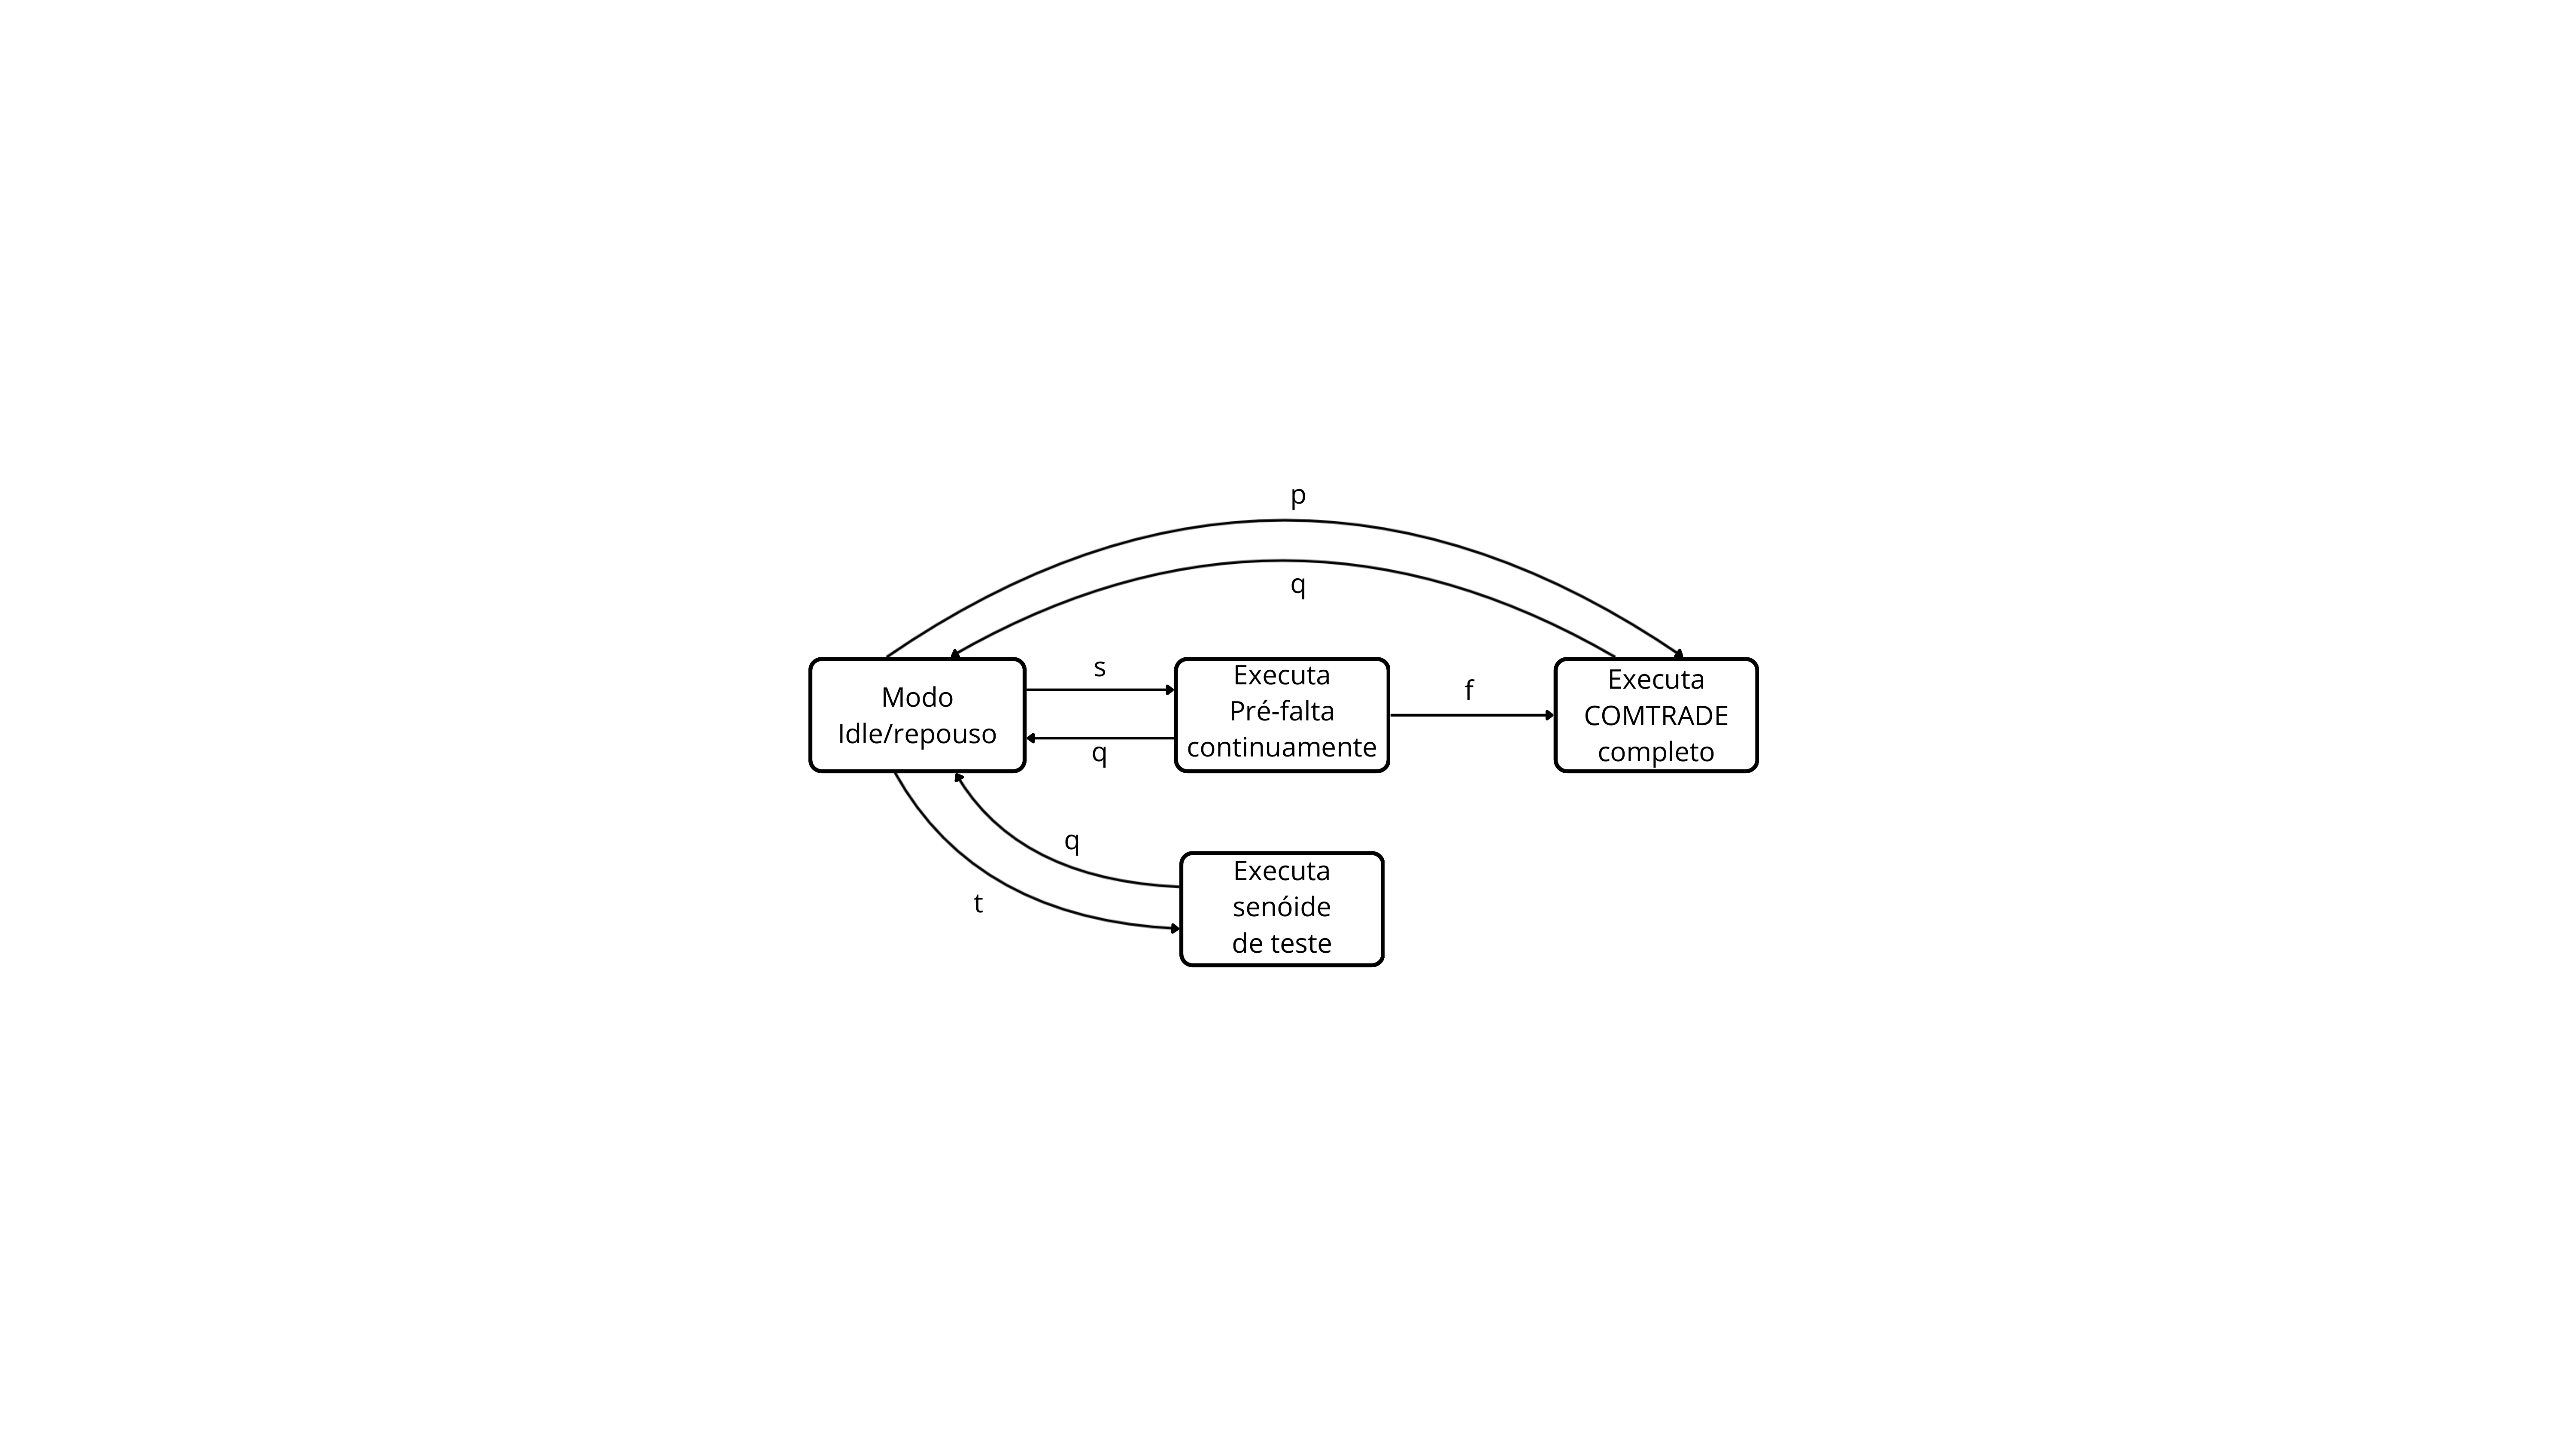
\includegraphics[
    width=0.75\textwidth,
    trim=450pt 265pt 450pt 265pt,
    clip
  ]{figuras/maquina_de_estado_v2_limpo.png}
  \legend{Fonte: Autoria própria.}
\end{figure}

Em qualquer estado de reprodução, o comando \texttt{q} interrompe o modo corrente, limpa o estado de reprodução e retorna o sistema a \textit{Idle}/repouso. O comando \texttt{x} possui precedência global: independentemente do estado, interrompe a execução, retorna a unidade geradora ao repouso e encerra o terminal Python.

\section{Interface Python da unidade receptora}

O programa \texttt{run\_embedded\_receiver.py} transforma o JSON e os argumentos da linha de comando em comandos \texttt{cfg chave valor}. Primeiro, carrega os blocos \texttt{receiver\_recommendation} e \texttt{comtrade\_reference}. Em seguida, prepara a taxa de amostragem, escalas, valores nominais, frequência de referência e limites admissíveis de frequência. As escalas \texttt{v\_scale\_eng\_per\_volt} e \texttt{i\_scale\_eng\_per\_volt}, originalmente vindas do JSON, podem ser multiplicadas pelos argumentos \texttt{--v-scale-correction} e \texttt{--i-scale-correction}. Na ausência desses argumentos, ambos os fatores são iguais a 1 e o comportamento permanece idêntico ao uso direto do JSON. As combinações de argumentos mais usuais são reunidas no Apêndice \ref{ap:comandos-execucao}.

A correção de escala é determinada durante a pré-falta contínua. Com a geradora no modo \texttt{s}, o comando \texttt{status} da receptora fornece as magnitudes $V_1$ e $I_1$ estimadas pela DFT. Comparando essas magnitudes aos valores nominais eficazes do JSON, obtêm-se

\begin{equation}
  C_V=\frac{V_{\mathrm{nom,rms}}}{V_{1,\mathrm{pre}}}, \qquad
  C_I=\frac{I_{\mathrm{nom,rms}}}{I_{1,\mathrm{pre}}},
  \label{eq:correcao-escala-receptor}
\end{equation}

em que $C_V$ e $C_I$ são os fatores usados, respectivamente, em \texttt{--v-scale-correction} e \texttt{--i-scale-correction}. Por exemplo, se a pré-falta de um registro nominal for reconstruída como $1{,}27$ pu, utiliza-se um fator próximo de $1/1{,}27$. Essa etapa corrige erro de ganho aproximadamente constante da cadeia analógica; ela não corrige saturação, recorte, troca de canais, erro de fase, falta de terra comum ou uso de JSON pertencente a outro COMTRADE.

Os ajustes são definidos pelos argumentos fornecidos no terminal. A opção \texttt{--over-current} configura conjuntamente o grupo 50/51; \texttt{--distance} configura a função 21; \texttt{--under-voltage} e \texttt{--over-voltage} configuram, respectivamente, 27 e 59; e \texttt{--directional-67} seleciona \texttt{forward} ou \texttt{reverse} e habilita a supervisão direcional. Desse modo, os grupos de proteção 21, 27, 50/51 e 59 podem ser solicitados separadamente ou combinados livremente na mesma linha de comando. A função 67 também é opcional: quando omitida, os grupos selecionados operam de forma não direcional; quando incluída, supervisiona todas as proteções também selecionadas naquele ensaio. Grupos não solicitados são explicitamente desabilitados, evitando ajustes residuais de uma execução anterior. Como a decisão implementada utiliza o sinal da potência ativa de pré-falta, a interface não solicita ângulo de máximo torque nem abertura de janela; esses parâmetros pertencem à extensão angular proposta para trabalhos futuros.

Ao abrir a porta serial, o \textit{script} aguarda \path{READY_EMBEDDED_RX}. Em seguida, envia \texttt{stop} e \texttt{resettrip} e somente então transmite os ajustes. Para cada parâmetro, exige uma confirmação do tipo \texttt{ACK cfg chave=valor}. Após todas as confirmações, envia \texttt{start}. Essa sequência impede que a proteção opere com uma configuração parcialmente atualizada.

Durante a execução, somente mensagens de evento, erro ou estado são exibidas. O encerramento por \texttt{Ctrl+C} produz o comando \texttt{stop}; os \textit{trips} permanecem retidos na ESP32 até \texttt{resettrip} ou reinicialização.

\section{Firmware da ESP32 receptora}

\subsection{Aquisição e conversão das entradas}

A aquisição é executada no laço principal segundo um período calculado por $10^6/f_s$ microssegundos. Em cada instante, são efetuadas oito conversões consecutivas em cada canal e calculada a média aritmética. O uso da média reduz parte da dispersão do ADC, embora não substitua uma calibração metrológica da entrada.

O código ADC é convertido para volts por

\begin{equation}
  v_{\mathrm{ADC}}=\frac{d_{\mathrm{ADC}}}{4095}\,3{,}3.
\end{equation}

Essa conversão é uma aproximação conveniente para reconstrução em tempo real. Na prática, a resposta do ADC interno da ESP32, especialmente com atenuação \texttt{ADC\_11db}, pode apresentar não linearidade e fundo de escala efetivo diferente da referência ideal. Por esse motivo, as grandezas absolutas usadas por 27, 59, 50 e 51 devem ser verificadas em pré-falta e, quando necessário, ajustadas pelos fatores de correção enviados pelo \textit{script} receptor. A função 21 tende a ser menos sensível a um erro comum de ganho, pois utiliza a razão $Z=V_1/I_1$; entretanto, a calibração continua necessária para manter coerência entre todas as funções.

Valores próximos de 0 ou 4095 ativam o indicador de saturação. Como o sinal possui deslocamento de aproximadamente \SI{1,65}{\volt}, o \textit{firmware} estima separadamente os \textit{offsets} de tensão e corrente por um filtro recursivo:

\begin{equation}
  \bar{v}[k]=\bar{v}[k-1]+\alpha\left(v[k]-\bar{v}[k-1]\right),
  \qquad \alpha=\frac{\Delta t}{\tau},
  \label{eq:filtro-offset}
\end{equation}

com constante de tempo padrão $\tau=\SI{1}{\second}$. As grandezas instantâneas são recuperadas por

\begin{equation}
  V[k]=(v_{\mathrm{ADC}}[k]-\bar{v}[k])K_V, \qquad
  I[k]=(i_{\mathrm{ADC}}[k]-\bar{i}[k])K_I,
  \label{eq:reconstrucao-engenharia}
\end{equation}

em que $K_V$ e $K_I$ são lidos do JSON. Como a geradora utiliza amplitude útil de \SI{1,55}{\volt}, esses fatores são calculados por $V_{\mathrm{clip}}/1{,}55$ e $I_{\mathrm{clip}}/1{,}55$.

O \textit{firmware} também estima um limite máximo de variação entre amostras a partir da amplitude nominal, da frequência e da taxa de amostragem. Saltos superiores a seis vezes a variação prevista são substituídos pelo valor anterior e o ciclo recebe uma marca de \textit{outlier}. Esse mecanismo evita que impulsos isolados dominem a DFT, mas deve ser acompanhado, pois uma filtragem excessiva também pode ocultar transitórios reais.

\subsection{Delimitação dos ciclos e controle de qualidade}

Os ciclos são delimitados pelas passagens ascendentes da tensão por zero após a remoção do \textit{offset}. Uma histerese impede múltiplas detecções produzidas por ruído próximo ao cruzamento. Entre duas passagens, o \textit{firmware} armazena até 160 pares de amostras.

Um ciclo é considerado inválido se possuir menos de oito amostras ou se a frequência estimada estiver fora da faixa configurada. São mantidos sinalizadores independentes para saturação do ADC, amostra discrepante, ciclo incompleto e frequência fora da faixa. Esses indicadores são apresentados no campo \texttt{qf} do comando \texttt{status} e devem ser consultados durante a validação.

A frequência é calculada diretamente pelo intervalo $T_c$ entre passagens por zero:

\begin{equation}
  f=\frac{1}{T_c}.
\end{equation}

Para um registro de \SI{60}{\hertz} amostrado a \SI{1000}{\hertz}, cada ciclo contém aproximadamente 16 ou 17 amostras. Embora seja suficiente para a demonstração, essa quantidade limita a resolução temporal e a representação de componentes de maior frequência.

\subsection{Estimação da componente fundamental}

Ao final de cada ciclo válido, a DFT de um ciclo é aplicada separadamente a tensão e corrente. Para $N$ amostras, as componentes real e imaginária são

\begin{equation}
  X_R=\sum_{k=0}^{N-1}x[k]\cos\left(\frac{2\pi k}{N}\right), \qquad
  X_I=-\sum_{k=0}^{N-1}x[k]\sin\left(\frac{2\pi k}{N}\right).
\end{equation}

A magnitude eficaz e o ângulo são calculados por

\begin{equation}
  |X_1|_{\mathrm{rms}}=\frac{\sqrt{2}}{N}\sqrt{X_R^2+X_I^2}, \qquad
  \angle X_1=\operatorname{atan2}(X_I,X_R).
  \label{eq:dft-fundamental-implementacao}
\end{equation}

Como a janela é definida por cruzamentos de zero e utiliza exatamente as amostras do ciclo observado, a DFT acompanha variações moderadas de frequência. O algoritmo fornece $V_1$, $I_1$, seus ângulos e a diferença angular necessária para o cálculo de impedância e potência.

\subsection{Normalização opcional pela pré-falta}

Quando a opção \texttt{normalize\_to\_comtrade} está ativa, o \textit{firmware} coleta dez ciclos válidos de pré-falta. Somente ciclos cujas magnitudes superem o limite mínimo configurado são aceitos. A mediana das magnitudes é comparada aos valores nominais do JSON, originando os ganhos

\begin{equation}
  G_V=\frac{V_{\mathrm{nom,rms}}}{\operatorname{med}(V_{1,\mathrm{pre}})}, \qquad
  G_I=\frac{I_{\mathrm{nom,rms}}}{\operatorname{med}(I_{1,\mathrm{pre}})}.
\end{equation}

Depois da estabilização, $V_1$ e $I_1$ são multiplicados por esses ganhos. A normalização compensa erros de ganho aproximadamente constantes da cadeia DAC--ADC. Ela é distinta dos fatores \texttt{--v-scale-correction} e \texttt{--i-scale-correction}: estes alteram a escala enviada ao \textit{firmware} antes do início do ensaio, enquanto a normalização é calculada internamente pela receptora a partir dos ciclos válidos observados. Em ambos os casos, a pré-falta deve estar estabilizada. Nenhum desses recursos corrige troca de canais, recorte, erro de fase, ausência de terra comum ou configuração pertencente a outro COMTRADE.

\section{Implementação das funções de proteção}

As proteções são avaliadas uma vez por ciclo elétrico válido. Os temporizadores acumulam a duração medida de cada ciclo, em vez de presumir um período fixo de \SI{16,67}{\milli\second}. Os estados de \textit{trip} são retidos. Após a primeira indicação geral de abertura, os resultados permanecem disponíveis até a limpeza explícita.

\subsection{Sobrecorrente instantânea e temporizada -- ANSI 50/51}

Os níveis de atuação são derivados da corrente nominal do JSON:

\begin{equation}
  I_{50}=I_N\left(1+\frac{p_{50}}{100}\right), \qquad
  I_{51}=I_N\left(1+\frac{p_{51}}{100}\right).
  \label{eq:pickup-sobrecorrente}
\end{equation}

Assim, na implementação atual, os argumentos percentuais representam acréscimo sobre a corrente nominal, e não múltiplos diretos ou percentuais absolutos de $I_N$. Essa semântica deve ser explicitada ao definir os ensaios, pois difere de algumas interfaces de relés comerciais.

Quando $I_1\geq I_{50}$, a função 50 atende ao seu critério instantâneo. Quando $I_1\geq I_{51}$, a função 51 entra em \textit{pickup} e acumula o tempo dos ciclos até o atraso ajustado. O retorno ocorre abaixo de $0{,}95I_{51}$ enquanto não houver \textit{trip}, introduzindo uma histerese de 5\%. A curva implementada é de tempo definido; não há, nesta versão, curva inversa IEC ou IEEE. Se a função 67 estiver habilitada, o \textit{trip} da 50 e o avanço do temporizador da 51 também exigem permissão direcional; sem a 67, ambas operam apenas pelos critérios de corrente e tempo.

\subsection{Subtensão e sobretensão -- ANSI 27/59}

Os níveis instantâneos e temporizados são derivados da tensão nominal eficaz:

\begin{equation}
  V_{27,i}=V_N\frac{p_{27,i}}{100}, \qquad
  V_{27,t}=V_N\left(1-\frac{p_{27,t}}{100}\right),
\end{equation}

\begin{equation}
  V_{59,i}=V_N\left(1+\frac{p_{59,i}}{100}\right), \qquad
  V_{59,t}=V_N\left(1+\frac{p_{59,t}}{100}\right).
\end{equation}

Cada função de tensão possui dois estágios. Para a função 27, o primeiro argumento define a tensão remanescente crítica, em porcentagem de $V_N$, para atuação instantânea; o segundo define uma queda percentual moderada, de modo que o \textit{pickup} temporizado é $V_N(1-p_{27,t}/100)$. Assim, \texttt{--under-voltage 50 10 0.20} produz \textit{trip} instantâneo quando $V_1\leq0{,}50V_N$ e \textit{trip} temporizado, após \SI{0,20}{\second}, quando $V_1\leq0{,}90V_N$ sem atingir o estágio instantâneo.

Para a função 59, os dois percentuais representam elevações sobre $V_N$. O comando \texttt{--over-voltage 50 10 0.20} produz \textit{trip} instantâneo quando $V_1\geq1{,}50V_N$ e \textit{trip} temporizado, após \SI{0,20}{\second}, quando $V_1\geq1{,}10V_N$ sem atingir o estágio instantâneo. O \textit{pickup} é reconhecido no primeiro ciclo fasorial válido; ``instantâneo'' significa ausência de atraso intencional adicional. O retorno dos estágios temporizados utiliza histerese de 3\%. Quando a função 67 está habilitada, tanto o \textit{trip} instantâneo quanto o avanço dos temporizadores exigem permissão direcional.

\subsection{Proteção de distância -- ANSI 21}

A impedância aparente monofásica é calculada por

\begin{equation}
  Z_{\mathrm{ap}}=\frac{V_1}{I_1}, \qquad
  \theta_Z=\angle V_1-\angle I_1,
\end{equation}

e convertida em coordenadas cartesianas:

\begin{equation}
  R=|Z_{\mathrm{ap}}|\cos\theta_Z, \qquad
  X=|Z_{\mathrm{ap}}|\sin\theta_Z.
\end{equation}

A avaliação só ocorre se $I_1$ superar 5\% da corrente nominal, reduzindo instabilidade causada por divisões por correntes muito pequenas. Os alcances são calculados a partir da impedância total da linha:

\begin{equation}
  Z_1=Z_L\frac{p_1}{100}, \qquad
  Z_2=Z_L\frac{p_2}{100}.
\end{equation}

Cada zona possui característica mho. Para alcance $Z_R$ e ângulo de linha $\theta_L$, o círculo tem raio $Z_R/2$ e centro

\begin{equation}
  C_R=\frac{Z_R}{2}\cos\theta_L, \qquad
  C_X=\frac{Z_R}{2}\sin\theta_L.
\end{equation}

O ponto $(R,X)$ opera quando

\begin{equation}
  (R-C_R)^2+(X-C_X)^2\leq\left(\frac{Z_R}{2}\right)^2.
  \label{eq:mho-operacao}
\end{equation}

A zona 1 é instantânea. A zona 2 exclui pontos já classificados na zona 1 e utiliza temporização de tempo definido. Para o retorno da zona 2, é empregado alcance de 105\% do ajuste, produzindo histerese. O \textit{firmware} também informa a distância aparente como percentual de $Z_L$, embora esse percentual seja uma estimativa baseada no módulo da impedância e não uma localização rigorosa para todos os tipos de falta.

\subsection{Supervisão direcional -- ANSI 67}
\label{sec:hierarquia-protecoes}

A função 67 foi implementada como supervisão permissiva comum às funções 21, 27, 50, 51 e 59. Essa associação corresponde à filosofia adotada no projeto e não deve ser interpretada como condição obrigatória para toda aplicação de proteção. Sua finalidade não é substituir o critério próprio de cada função, mas acrescentar uma condição direcional quando a 67 e uma ou mais proteções atuantes forem habilitadas no mesmo ensaio. Para $F\in\{21,27,50,51,59\}$, a lógica executada pode ser expressa por

\begin{equation}
  \operatorname{trip}_F=\operatorname{op}_F\land
  \left(\neg E_{67}\lor G_{67}\right),
  \label{eq:permissivo-67}
\end{equation}

em que $\operatorname{op}_F$ representa o atendimento dos critérios próprios da função, $E_{67}$ indica que a supervisão direcional está habilitada e $G_{67}$ representa a permissão direcional. Dessa forma, a proteção opera normalmente quando a função 67 está desabilitada; quando a supervisão está ativa, a ausência de permissão bloqueia a atuação, mesmo que o \textit{pickup} da função supervisionada tenha ocorrido.

O critério direcional disponível no \textit{firmware} estima a potência ativa por

\begin{equation}
  P_{67}=|V_1||I_1|\cos(\angle V_1-\angle I_1).
\end{equation}

Enquanto nenhuma das funções supervisionadas está em \textit{pickup}, valores de potência cujo módulo supera o limiar configurado atualizam a referência de pré-falta. Potência de pré-falta positiva representa sentido direto e potência negativa, sentido reverso. O estado direcional é calculado uma única vez a cada ciclo válido e compartilhado pelos blocos 21, 27, 50, 51 e 59.

Para a função 21, a falta de permissão bloqueia tanto o \textit{trip} instantâneo da zona 1 quanto a temporização da zona 2. Na 50, bloqueia o \textit{trip} instantâneo; na 51, impede o avanço do temporizador. Para 27 e 59, o \textit{pickup} permanece observável, mas a ausência de permissão bloqueia o estágio instantâneo e mantém em zero o temporizador do estágio temporizado. Quando a permissão passa a existir e a condição de \textit{pickup} persiste, o estágio instantâneo atua no primeiro ciclo válido permitido, enquanto a temporização do estágio moderado começa a partir de zero. Essa regra exige simultaneamente o critério próprio da proteção, a condição temporal correspondente e, quando solicitada, a condição direcional da função 67.

Na implementação avaliada, a decisão direcional baseia-se no sinal da potência ativa de pré-falta. A adoção futura de um comparador angular explícito com torque polarizante permitirá investigar outras filosofias direcionais e aplicar sua saída permissiva, de maneira uniforme, a todas as funções supervisionáveis.

\subsection{Eventos, retenção e prioridade lógica}

Quando habilitada, a emissão de eventos informa transições de \textit{pickup}, temporização, retorno, bloqueio e \textit{trip}. Mensagens de temporização são limitadas por um intervalo mínimo, reduzindo a ocupação da serial. Ao surgir qualquer \textit{trip}, uma mensagem geral \texttt{BREAKER TRIP} reúne as fontes ativas.

Os \textit{trips} permanecem retidos até o comando \texttt{resettrip}. Esse comportamento reproduz, de forma simplificada, a necessidade de reconhecimento de uma atuação. As saídas agregadas dos GPIO26 e GPIO25 são acionadas somente após o \textit{trip}, respectivamente instantâneo ou temporizado; \textit{pickups} e temporizadores em andamento permanecem observáveis pela interface serial.

\section{Protocolo de configuração e supervisão da receptora}

\begin{table}[H]
  \centering
  \small
  \caption{Comandos principais do \textit{firmware} receptor.}
  \label{tab:comandos-receptor}
  \begin{tabular}{ll}
    \toprule
    Comando & Finalidade \\
    \midrule
    \texttt{cfg chave valor} & Alterar um parâmetro e recalcular os ajustes derivados \\
    \texttt{start} & Iniciar aquisição e avaliação das proteções \\
    \texttt{stop} & Suspender aquisição e proteção \\
    \texttt{status} & Exibir fasores, frequência, impedância, qualidade e \textit{trips} \\
    \texttt{resettrip} & Limpar temporizadores, \textit{trips} e saídas retidas \\
    \texttt{testrelays} & Acionar sequencialmente as quatro saídas de proteção \\
    \bottomrule
  \end{tabular}
  \legend{Fonte: Autoria própria.}
\end{table}

O comando \texttt{status} é especialmente útil para a implementação e a depuração. Ele apresenta quantidade de amostras e ciclos, $V_1$, $I_1$, frequência, validade da DFT, ganhos de normalização, impedância, resistência, reatância, estados das zonas, temporizador da zona 2, permissão direcional, \textit{trips} e indicadores de qualidade. A consulta a esse comando durante a pré-falta faz parte do procedimento operacional descrito no Apêndice \ref{ap:comandos-execucao}.

\section{Montagem e execução integrada}

A montagem completa e a bancada foram apresentadas nas Figuras \ref{fig:sistema-completo} e \ref{fig:bancada-testes}, no capítulo de Metodologia. Na execução integrada, as duas placas são conectadas ao computador por portas seriais distintas. Depois do \textit{upload} e do processamento do COMTRADE, a receptora é configurada com o JSON recém-gerado. A geradora deve permanecer inicialmente em pré-falta contínua; nessa condição, verifica-se se $V_1$ e $I_1$ medidos pela receptora coincidem com os valores nominais do JSON. Quando houver desvio sistemático de ganho, são aplicadas as correções de escala no comando da receptora. Somente após essa verificação são liberadas as proteções e, posteriormente, o evento completo.

\subsection{Execução dos comandos de geração e recepção}

A execução utiliza dois terminais. No primeiro, aberto no diretório da unidade geradora, o par COMTRADE é transmitido à ESP32 conectada em \path{/dev/ttyUSB0}. O argumento \texttt{--receiver-config} define o JSON que será compartilhado com a receptora:

\begin{verbatim}
cd generator/python/embedded_generator
python3 run_embedded_generator.py \
  --cfg samples/sample_3/export.cfg \
  --bdat samples/sample_3/export.bdat \
  --port /dev/ttyUSB0 \
  --baud 921600 \
  --receiver-config config.json
\end{verbatim}

Depois de \texttt{READY\_PLAYBACK}, o terminal aceita os comandos de reprodução. A sequência usual é \texttt{s}, para manter a pré-falta contínua, seguida de \texttt{f}, para encadear o evento COMTRADE completo. Os comandos \texttt{q} e \texttt{x} interrompem a reprodução, sendo que o segundo também encerra a interface.

No segundo terminal, aberto no diretório da receptora, o JSON recém-criado é enviado com os ajustes das proteções. O exemplo seguinte habilita normalização pela pré-falta, proteção de distância, supervisão direcional e exibição dos eventos:

\begin{verbatim}
cd receiver/python/embedded_receiver
CONFIG=../../../generator/python/embedded_generator/config.json
python3 run_embedded_receiver.py \
  --config "$CONFIG" \
  --port /dev/ttyUSB1 \
  --v-scale-correction 0.785 \
  --i-scale-correction 0.780 \
  --normalize-to-comtrade \
  --distance 52.12496 80 120 0.05 \
  --distance-line-angle 86.636 \
  --directional-67 forward \
  --protection-events
\end{verbatim}

Nesse comando, \texttt{52.12496} é o módulo da impedância da linha em ohms; \texttt{80} e \texttt{120} são os alcances percentuais das zonas 1 e 2; e \texttt{0.05} é o atraso da zona 2 em segundos. O argumento \texttt{--distance-line-angle} orienta os círculos mho, enquanto \texttt{--directional-67 forward} seleciona o sinal positivo da potência ativa de pré-falta como sentido permitido. Os fatores \texttt{--v-scale-correction} e \texttt{--i-scale-correction} são exemplos de correção obtidos pela razão entre as magnitudes nominais do JSON e as magnitudes medidas em pré-falta; em outra montagem ou outra placa, esses valores devem ser recalculados. Os nomes das portas seriais devem ser adaptados à enumeração observada no sistema operacional. O Apêndice \ref{ap:comandos-execucao} reúne as demais combinações e descreve os argumentos principais.

Durante esse processo, qualquer função habilitada pode produzir \textit{pickup}, temporização, retorno ou \textit{trip}. Os eventos das funções 27, 59, 50, 51 e 21 são discriminados na comunicação serial. O painel físico fornece uma indicação geral para qualquer \textit{trip}, duas indicações comuns de bloqueio e permissão da supervisão 67 e duas indicações agregadas para \textit{trips} instantâneos e temporizados.

\section{Tratamento de falhas e mecanismos de diagnóstico}

A implementação contém verificações em diferentes pontos do fluxo. Na geradora, são detectadas ausência do MCP4728, falha do LittleFS, falha de alocação, formato COMTRADE incompatível, \textit{layout} binário inválido, \textit{timeout} de \textit{upload}, falta de quadros e esvaziamento do \textit{buffer}. Na receptora, são sinalizados saturação, amostras discrepantes, ciclo incompleto, frequência inválida e comandos desconhecidos.

As mensagens iniciadas por \texttt{READY}, \texttt{STATUS}, \texttt{ACK}, \texttt{OK}, \texttt{WARN} e \texttt{ERR} formam uma interface textual de diagnóstico. Embora simples, essa padronização permite distinguir prontidão, progresso, confirmação e falha. Os \textit{scripts} Python interrompem a sequência quando recebem \texttt{ERR} ou quando uma confirmação não chega dentro do prazo.

Como evolução do protocolo, trabalhos futuros poderão acrescentar CRC ao \textit{upload} e armazenar no JSON um identificador do \texttt{.cfg} e do \texttt{.bdat}, ampliando a rastreabilidade dos arquivos utilizados em cada ensaio.

\section{Limitações técnicas e operacionais}
\label{sec:limitacoes-tecnicas}

\subsection{Taxa de amostragem e capacidade de processamento}

A taxa de \SI{1000}{amostras\per\second} foi estabelecida empiricamente como limite operacional do protótipo a partir da observação da saída analógica da ESP32 geradora. Até esse valor, a temporização das amostras preservou adequadamente a frequência de \SI{60}{\hertz} do sistema simulado. Acima dele, as atualizações começaram a perder sincronismo e o período da forma de onda reproduzida deixou de corresponder de maneira estável ao período de \SI{16,67}{\milli\second} esperado para \SI{60}{\hertz}. A taxa adotada também é usada na senoide interna de teste, constitui o valor inicial da receptora e fornece aproximadamente 16,7 amostras por ciclo.

O uso de uma taxa superior reduz o intervalo disponível entre atualizações. A \SI{1000}{amostras\per\second}, cada quadro dispõe nominalmente de \SI{1}{\milli\second}. Nesse período, a unidade geradora precisa retirar o quadro do \textit{buffer}, aguardar sua marca de tempo e atualizar os quatro canais do MCP4728 pelo barramento I\textsuperscript{2}C configurado em \SI{1}{\mega\hertz}. Simultaneamente, as tarefas de controle precisam manter o \textit{buffer} abastecido. Na receptora, cada instante envolve oito conversões ADC para tensão, oito para corrente, cálculo das médias, remoção de \textit{offset}, aplicação das escalas, verificação de qualidade e armazenamento da amostra. Ao final do ciclo elétrico ainda são executadas a DFT e as funções de proteção. Assim, o aumento da taxa diminui a margem temporal para todas essas operações e torna a execução mais sensível à latência do I\textsuperscript{2}C, ao tempo das conversões ADC, ao escalonamento do FreeRTOS e às interrupções do sistema.

Embora o limite tenha sido identificado experimentalmente na bancada, o código não rejeita automaticamente registros com taxas superiores. Além disso, a observação realizada caracteriza o limite operacional da implementação completa, mas não isola o tempo consumido por cada componente nem estabelece uma barreira física absoluta da ESP32 ou do MCP4728. O comportamento observado é compatível com a redução da margem entre quadros: quando o processamento e a atualização do DAC consomem tempo próximo ou superior ao intervalo solicitado, os atrasos acumulados distorcem a base de tempo e, consequentemente, a frequência reproduzida. A operação acima de \SI{1000}{amostras\per\second} exigiria otimização e nova validação, com medição dos intervalos de atualização, contagem de underflows e comparação da frequência solicitada com a frequência efetivamente presente na saída.

\subsection{Buffer, memória e continuidade temporal}

O \textit{buffer} circular da geradora contém 4096 quadros. Sem interpolação, essa capacidade corresponde a aproximadamente \SI{4,096}{\second} a \SI{1000}{amostras\per\second}, \SI{2,048}{\second} a \SI{2000}{amostras\per\second} e \SI{1,024}{\second} a \SI{4000}{amostras\per\second}. O \textit{buffer} funciona como uma fila de desacoplamento entre a tarefa de controle e a tarefa do DAC; ele não representa, necessariamente, o limite de duração do registro, pois os quadros do evento completo são alocados separadamente na memória e inseridos na fila à medida que são consumidos.

A interpolação também altera a ocupação efetiva. Quando a diferença entre códigos consecutivos supera 64 unidades e o intervalo permite, um intervalo original pode ser dividido em até quatro quadros, respeitando o passo temporal mínimo de \SI{250}{\micro\second}. No caso extremo, a mesma capacidade circular passa a representar apenas 1024 intervalos originais. Além disso, a expansão requer um novo bloco de memória para os quadros interpolados. O \textit{firmware} tenta alocá-lo primeiro em PSRAM e, na indisponibilidade desta, na memória interna; se a alocação falhar, emite \texttt{WARN code=INTERP\_ALLOC} e preserva os quadros sem expansão. Dessa forma, registros longos e elevada incidência de interpolação aumentam o consumo de memória e podem reduzir a suavização esperada.

Quando a tarefa do DAC encontra a fila vazia, incrementa o contador de \textit{underflow}, interrompe o estado de reprodução e aguarda novos quadros. Se uma atualização ocorre com atraso superior a quatro períodos do quadro, o relógio de reprodução é parcialmente corrigido para reduzir o atraso acumulado. Esse mecanismo evita crescimento ilimitado da defasagem, mas não recupera os instantes que já deixaram de ser atendidos. Consequentemente, um \textit{underflow} ou atraso excessivo representa perda de regularidade temporal, mesmo que todos os valores do registro permaneçam armazenados e venham a ser processados posteriormente.

Na receptora, quando o laço principal está atrasado mais de quatro períodos, a próxima marca de aquisição é reposicionada a partir do instante corrente. Essa decisão impede uma sequência de leituras atrasadas em rajada, porém implica que instantes intermediários não são adquiridos. O \textit{firmware} sinaliza ciclos incompletos e mantém no máximo 160 pares de amostras por ciclo. Esse limite é confortável no ponto de operação de \SI{1000}{amostras\per\second}, mas taxas elevadas ou frequências fundamentais menores aumentam o número de amostras por ciclo e podem atingir a capacidade do vetor.

\subsection{Restrições de formato e da cadeia analógica}

O processador COMTRADE foi delimitado a registros binários e utiliza os dois primeiros canais analógicos como tensão e corrente. O \textit{parser} lê até 160 linhas do arquivo \texttt{.cfg} e a implementação não contempla todas as combinações previstas pela norma, múltiplas taxas de amostragem no mesmo registro nem reprodução trifásica completa. Arquivos fora desse subconjunto precisam ser convertidos e reorganizados antes do ensaio.

Na cadeia analógica, o DAC e o ADC possuem resolução nominal de 12 bits, mas a resolução efetiva é afetada por ruído, não linearidade, variação da referência, \textit{offset} e montagem em protoboard. O deslocamento de \SI{1,65}{\volt} permite representar grandezas alternadas dentro da faixa unipolar, mas reduz a margem até os limites de saturação. A média de oito leituras, a estimação recursiva do \textit{offset} e os fatores de correção de escala atenuam parte da dispersão e do erro de ganho, sem substituir condicionamento analógico, isolamento e calibração metrológica. Por isso, a plataforma é adequada à demonstração didática e à comparação funcional das proteções, mas seus resultados não devem ser interpretados como equivalentes aos de um relé comercial ou de um sistema de aquisição certificado.

\section{Conclusão}

A implementação distribuiu as tarefas críticas entre duas ESP32. A unidade geradora recebe e armazena o COMTRADE, calcula referências, converte grandezas de engenharia em quadros temporizados e atualiza o MCP4728 por uma tarefa dedicada. A unidade receptora digitaliza os sinais, remove o nível médio, reconstrói as grandezas, estima fasores por DFT e avalia as funções de proteção a cada ciclo válido.

O \texttt{config.json} mantém a coerência de escala entre as duas unidades, enquanto os protocolos seriais garantem que arquivos e parâmetros sejam confirmados antes da execução. A combinação de \textit{buffer} circular, tarefas FreeRTOS, controle de qualidade das amostras, retenção de \textit{trips} e saídas físicas permite que o protótipo represente, de maneira observável, o caminho entre uma oscilografia simulada e a decisão de proteção. Os trechos de código e comandos apresentados no Apêndice \ref{ap:comandos-execucao} documentam esse fluxo de forma resumida; a implementação integral permanece no repositório do projeto.
